\section{Tomada de Decisão e Relação de Causalidade}

\begin{frame}{Tomada de Decisão Visual}
    \begin{columns}
        \begin{column}{0.5\textwidth}
            \textbf{Análise do Histograma Nulo:}
            \begin{itemize}
                \item O histograma mostra os valores da estatística de teste esperados sob a hipótese nula $H_0$.
                \item O valor observado de $0.475$ está marcado com a linha tracejada vermelha.
                \item Apenas uma proporção muito pequena das permutações (dourado) resultou em diferenças maiores ou iguais à observada.
                \item O desvio é muito extremo para ser explicado pelo acaso.
            \end{itemize}
        \end{column}
        \begin{column}{0.5\textwidth}
            \centering
            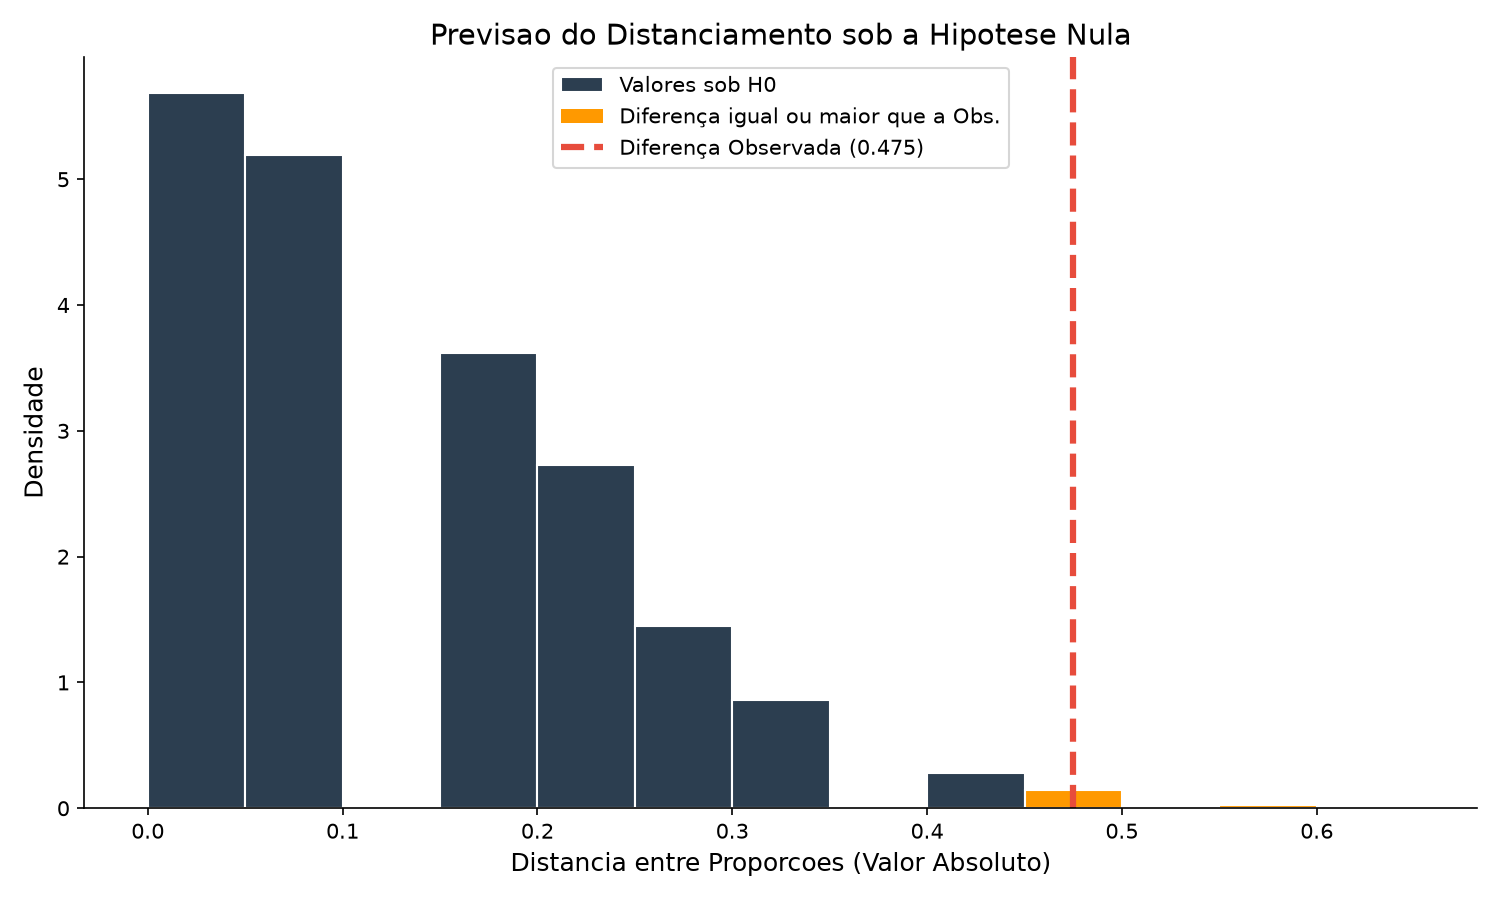
\includegraphics[width=\textwidth]{01_causalidade_histograma.png}
        \end{column}
    \end{columns}
\end{frame}

\begin{frame}{Decisão Estatística e Causalidade}
    \begin{block}{Resultado do Teste no Ceará}
        \begin{itemize}
            \item P-valor empírico calculado: $0.0091$ ($0.91\%$).
            \item Regra de Decisão: Como o P-valor ($0.91\%$) é menor que o nível de significância convencional ($\alpha = 5\%$), \textbf{rejeitamos a hipótese nula $H_0$}.
            \item As evidências estatísticas sustentam a hipótese alternativa $H_1$.
        \end{itemize}
    \end{block}
    \begin{alertblock}{Inferência de Causalidade}
        Como a alocação dos 31 pacientes aos grupos Tratamento e Controle foi feita de forma estritamente aleatória (por sorteio), concluímos que o tratamento com Toxina Botulínica Tipo A (BTA) \textbf{causou} a melhora clínica nos pacientes.
    \end{alertblock}
    \centering
    \textit{A randomização distribuiu as variáveis ocultas igualmente entre os grupos, eliminando o confundimento e validando a relação de causa e efeito!}
\end{frame}
